\section*{Antwort}

S. Abbildung~\ref{fig:aufgabe2}.\\

\begin{figure}
    \centering
    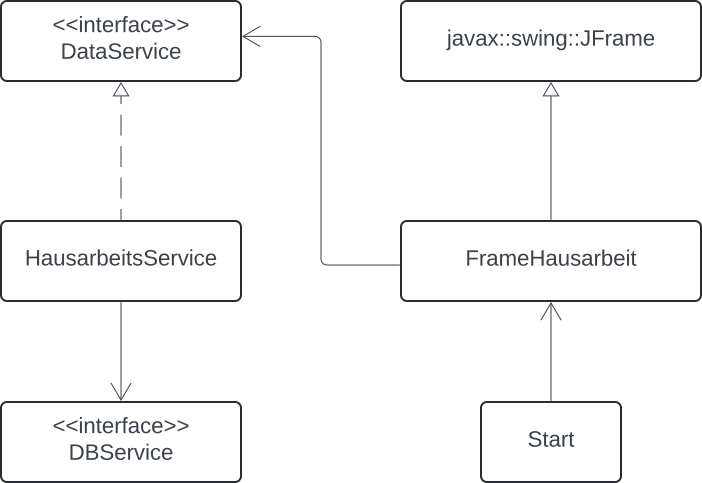
\includegraphics[scale=0.5]{chapters/aufgabe 2/img/aufgabe2}
    \caption{UML für den in Aufgabe 2 verkürzt dargestellten Quellcode. (Quelle: eigene)}
    \label{fig:aufgabe2}
\end{figure}

\noindent
Da der Quellcode in der Aufgabe verkürzt dargestellt ist, kann keine genaue Aussage zur Multiplizität getroffen werden - es geht aus dem Quelltext also nicht \textit{eindeutig} hervor, ob es sich bei den Assoziationen um \textbf{Kann}- oder \textbf{Muss}-Beziehungen handelt (vgl.~\cite[43]{Bal05}): Bei einer einseitigen \textbf{Muss}-Beziehung von Objekt A zu Objekt B muss bspw. die Beziehung zu Objekt B aufgebaut werden, sobald Objekt A erzeugt wird - hierzu fehlt aber zumindest der Konstruktor, der hierzu mehr Informationen liefern könnte. \\

\noindent
Würden wir die Multiplizität in dem resultierenden UML-Diagramm nicht angeben, wäre die Multiplizität implizit \code{[1]} ist\footnote{
    \textit{Fowler} empfiehlt diesbzgl. in \cite[39]{Fow03b} ``The default implicity of an attribute is [1]. Although this is true in the meta-model,you can't assume that an attribute in a diagram that's missing a multiplicity has a value of [1], as the diagram may be suppressing the multiplicity information. As a result, I prefer to explicitly state a [1] multiplicity if it's important.``
    }:
\blockquote[{\cite[19]{OMG17}}]{
If no multiplicity is shown on an association end, it implies a multiplicity of exactly 1. (\cite[19]{OMG17})
}.


\noindent
Auch die Navigierbarkeit der Assoziationen geht nicht \textit{eindeutig} für \textit{alle} Richtungen aus dem Quelltext hervor\footnote{
zur Verwendung der \textit{navigabilityNotation}- und \textit{nonNavigabilityNotation}-Notationselemente zur expliziten Darstellung der Navigierbarkeit s.~\cite[203]{OMG17}
}.\\
Indem wir alle Assoziationsrichtungen in dem resultierenden UML-Diagramm in jeweils eine Richtung angeben, erstellen wir in allen Fällen \textit{unidirektionale} Assoziationen: Bspw. können Objekte der Klasse \code{Start} über eine Referenz auf \code{FrameHausarbeit} zugreifen.\\
Wollten wir den umgekehrten Zugriff \textit{explizit} ausschließen, müssten wir noch die \textit{nonNavigableNotation}-Notation verwenden - ansonsten ist die andere Richtung \textit{undefiniert} (vgl.~\cite[285]{Bal05})\footnote{
    Bzgl. der in der UML-Spezifikation vereinbarten Konventionen bzgl. Navigierbarkeit s.a. ``Arrow notation is used to denote association end navigability. By definition, all class-owned association ends are navigable. By convention, all association-owned ends in the metamodel are not navigable.`` (\cite[18]{OMG17}) sowie ``An association with neither end marked by navigability arrows means that the association is navigable in both directions.`` (\cite[19]{OMG17})
}.\\

\noindent
Explizite Angaben zu Multiplizität und Navigierbarkeit können in einem \textbf{Feinentwurf} zur Vermeidung von Missverständnissen ergänzt werden (vgl.~\cite[415]{Bal05}). Auf den Feinentwurf folgt die Implementierung.